\chapter{Peripherals}

Most of the peripherals in \pulpissimo are connected to the \udma subsystem which
efficiently handles all the data-transfers autonoumsly.
The \udma must be programmed by the core via memory-mapped read and write operations to receive commands.

See the \udma documentation for more details under the \udma repository.

The GPIO, timers, event unit and event generator, debug and the FLLs are not connected to the \udma instead but to the APB bus.
Following a brief overview about these units is given.

\clearpage
\section{FLL}

\pulpissimo containts 3 FLLs. One FLL is meant for generating the clock for the
peripheral domain, one for the core domain (core, memories, event unit etc) and
one is meant for the cluster. The latter is not used.

All the FLLs can be bypassed by writing to the JTAG register before the reset
signal is asserted. See Section ~\ref{sec:soc_ctrl} for more details about the
bypass register.

\subsection{SoC FLL registers}
\begin{table}[htbp]
  \small
\begin{tabularx}{\textwidth}{|l|l|l|l|l|l|X|}
  \hline
  \textbf{Name} & \textbf{Address}  & \textbf{Size} & \textbf{Type} & \textbf{Access} & \textbf{Default} & \textbf{Description} \\
  \hline
  STATUS & \texttt{0x1A100000} & 32 & Status & R    & \texttt{0x00000000} & FLL status register \\
  \hline
  CFG1   & \texttt{0x1A100004} & 32 & Config & R/W    & \texttt{0x00000000} & FLL configuration 1 register \\
  \hline
  CFG2   & \texttt{0x1A100008} & 32 & Config & R/W    & \texttt{0x00000000} & FLL configuration 2 register \\
  \hline
  INTEG  & \texttt{0x1A10000C} & 32 & Config & R/W    & \texttt{0x00000000} & FLL integrator configuration register. \\
  \hline
\end{tabularx}
\caption{SoC FLL register table \label{tab:table_label}}
\end{table}


\regdoc{0x1A10\_0000}{0x0000\_0000}{STATUS}{
  \begin{bytefield}[endianness=big,bitwidth=2em]{16}
  \bitheader[lsb=16]{16-31} \\
  \bitbox{16}{\color{lightgray}\rule{\width}{\height}} \\[3ex]
  \bitheader{0-15} \\
  \bitbox{16}{MF}
  \end{bytefield}
}{
  \regitem{Bit 15-0}{MF}{R}{Current DCO multiplication factor value bitfield}
}

\regdoc{0x1A10\_0004}{0x0000\_0000}{CFG1}{
  \begin{bytefield}[endianness=big,bitwidth=2em]{16}
  \bitheader[lsb=16]{16-31} \\
  \bitbox{1}{\tiny CKM} \bitbox{1}{\tiny CKG} \bitbox{4}{CKDIV} \bitbox{10}{ICS} \\[3ex]
  \bitheader{0-15} \\
  \bitbox{16}{MFN}
  \end{bytefield}
}{
  \regitem{Bit 31}{CKM}{R/W}{FLL operation mode configuration bitfield
    \begin{itemize}
      \item 0b0: standalone
      \item 0b1: normal
    \end{itemize}}
  \regitem{Bit 30}{CKG}{R/W}{FLL output clock divider configuration
   \begin{itemize}
      \item 0b0: not gated
      \item 0b1: gated
    \end{itemize}}
  \regitem{Bit 29-26}{CKDIV}{R/W}{FLL output clock divider configuration}
  \regitem{Bit 25-16}{ICS}{R/W}{DCO input code in standalone}
  \regitem{Bit 15-0}{MFN}{R/W}{Target clock multiplication factor in normal mode}
}

\regdoc{0x1A10\_0008}{0x0000\_0000}{CFG2}{
  \begin{bytefield}[endianness=big,bitwidth=2em]{16}
  \bitheader[lsb=16]{16-31} \\
  \bitbox{1}{\tiny DITH} \bitbox{1}{\tiny OL} \bitbox{1}{\tiny CKSEL} \bitbox{1}{\color{lightgray}\rule{\width}{\height}} \bitbox{12}{LT} \\[3ex]
  \bitheader{0-15} \\
  \bitbox{6}{SCKL} \bitbox{6}{UCKL} \bitbox{4}{LG}
  \end{bytefield}
}{
  \regitem{Bit 31}{DITH}{R/W}{Dithering activation}
  \regitem{Bit 30}{CKM}{R/W}{Open loop when locked
    \begin{itemize}
      \item 0b0: disabled
      \item 0b1: enabled
    \end{itemize}}
  \regitem{Bit 29}{CKSEL}{R/W}{Configuration clock selection in standalone mode
    \begin{itemize}
      \item 0b0: DCO clock
      \item 0b1: Reference clock
    \end{itemize}}

  \regitem{Bit 27-16}{LT}{R/W}{Lock tolerance configuration. It is the margin
    around the multiplication factor within which the output clock is considered
    stable.}

  \regitem{Bit 15-10}{SCKL}{R/W}{Number of stable REFCLK cycles until LOCK
    assert in normal mode. Uppper 6 bits of LOCK assert counter target in
    standalone mode.}

  \regitem{Bit 9-4}{UCKL}{R/W}{Number of unstable REFCLK cycles until LOCK
    de-assert in normal mode. Lower 6 bits of LOCK assert counter target in
    standalone mode.}
  \regitem{Bit 3-0}{LG}{R/W}{FLL loop gain setting}
}


\regdoc{0x1A10\_000C}{0x0000\_0000}{INTEG}{
  \begin{bytefield}[endianness=big,bitwidth=2em]{16}
  \bitheader[lsb=16]{16-31} \\
  \bitbox{6}{\color{lightgray}\rule{\width}{\height}} \bitbox{10}{INTEG} \\[3ex]
  \bitheader{0-15} \\
  \bitbox{10}{FRAC} \bitbox{6}{\color{lightgray}\rule{\width}{\height}}
  \end{bytefield}
}{
  \regitem{Bit 25-16}{INTEG}{R/W}{Integer part of integrator state bitfield. It corresponds to DCO unit bits.}
  \regitem{Bit 15-6}{FRAC}{R/W}{Fractional part of integrator state bitfield. It corresponds to dither unit input.}
}


\clearpage
\section{APB GPIO}


\subsection{APB GPIO Registers}
{\small
\begin{tabularx}{\textwidth}{|l|l|l|l|l|l|X|}
  \hline
  \textbf{Name} & \textbf{Address}  & \textbf{Size} & \textbf{Type} & \textbf{Access} & \textbf{Default} & \textbf{Description} \\
  \hline
  PADDIR\_00\_31 & \texttt{0x1A101000} & 32 & Config & R/W & \texttt{0x00000000} & GPIO pad direction configuration register.\\
  \hline
  GPIOEN\_00\_31 & \texttt{0x1A101004} & 32 & Config & R/W & \texttt{0x00000000} & GPIO enable register.\\
  \hline
  PADIN\_00\_31 & \texttt{0x1A101008} & 32 & Config & R & \texttt{0x00000000} & GPIO pad input value register.\\
  \hline
  PADOUT\_00\_31 & \texttt{0x1A10100C} & 32 & Config & R/W & \texttt{0x00000000} & GPIO pad output value register.\\
  \hline
  PADOUTSET\_00\_31 & \texttt{0x1A101010} & 32 & Config & R/W & \texttt{0x00000000} & GPIO pad output set register.\\
  \hline
  PADOUTCLR\_00\_31 & \texttt{0x1A101014} & 32 & Config & R/W & \texttt{0x00000000} & GPIO pad output clear register.\\
  \hline
  INTEN\_00\_31 & \texttt{0x1A101018} & 32 & Config & R/W & \texttt{0x00000000} & GPIO pad interrupt enable configuration register.\\
  \hline
  INTTYPE\_00\_15 & \texttt{0x1A10101C} & 32 & Config & R/W & \texttt{0x00000000} & GPIO pad interrupt type gpio 0 to 15 register.\\
  \hline
  INTTYPE\_16\_31 & \texttt{0x1A101020} & 32 & Config & R/W & \texttt{0x00000000} & GPIO pad interrupt type gpio 16 to 31 register.\\
  \hline
  INTSTATUS\_00\_31 & \texttt{0x1A101024} & 32 & Status & R & \texttt{0x00000000} & GPIO pad interrupt status register.\\
  \hline
  PADCFG\_00\_07 & \texttt{0x1A101028} & 32 & Config & R/W & \texttt{0x00000000} & GPIO pad pin 0 to 7 configuration register.\\
  \hline
  PADCFG\_08\_15 & \texttt{0x1A10102C} & 32 & Config & R/W & \texttt{0x00000000} & GPIO pad pin 8 to 15 configuration register.\\
  \hline
  PADCFG\_16\_23 & \texttt{0x1A101030} & 32 & Config & R/W & \texttt{0x00000000} & GPIO pad pin 16 to 23 configuration register.\\
  \hline
  PADCFG\_24\_31 & \texttt{0x1A101034} & 32 & Config & R/W & \texttt{0x00000000} & GPIO pad pin 24 to 31 configuration register.\\
  \hline
  PADDIR\_32\_63 & \texttt{0x1A101038} & 32 & Config & R/W & \texttt{0x00000000} & GPIO pad direction configuration register.\\
  \hline
  GPIOEN\_32\_63 & \texttt{0x1A10103C} & 32 & Config & R/W & \texttt{0x00000000} & GPIO enable register.\\
  \hline
  PADIN\_32\_63 & \texttt{0x1A101040} & 32 & Config & R & \texttt{0x00000000} & GPIO pad input value register.\\
  \hline
  PADOUT\_32\_63 & \texttt{0x1A101044} & 32 & Config & R/W & \texttt{0x00000000} & GPIO pad output value register.\\
  \hline
  PADOUTSET\_32\_63 & \texttt{0x1A101048} & 32 & Config & R/W & \texttt{0x00000000} & GPIO pad output set register.\\
  \hline
  PADOUTCLR\_32\_63 & \texttt{0x1A10104C} & 32 & Config & R/W & \texttt{0x00000000} & GPIO pad output clear register.\\
  \hline
  INTEN\_32\_63 & \texttt{0x1A101050} & 32 & Config & R/W & \texttt{0x00000000} & GPIO pad interrupt enable configuration register.\\
  \hline
  INTTYPE\_32\_47 & \texttt{0x1A101054} & 32 & Config & R/W & \texttt{0x00000000} & GPIO pad interrupt type gpio 32 to 47 register.\\
  \hline
  INTTYPE\_48\_63 & \texttt{0x1A101058} & 32 & Config & R/W & \texttt{0x00000000} & GPIO pad interrupt type gpio 48 to 63 register.\\
  \hline
  INTSTATUS\_32\_63 & \texttt{0x1A10105C} & 32 & Status & R & \texttt{0x00000000} & GPIO pad interrupt status register.\\
  \hline
  PADCFG\_32\_39 & \texttt{0x1A101060} & 32 & Config & R/W & \texttt{0x00000000} & GPIO pad pin 32 to 39 configuration register.\\
  \hline
  PADCFG\_40\_47 & \texttt{0x1A101064} & 32 & Config & R/W & \texttt{0x00000000} & GPIO pad pin 40 to 47 configuration register.\\
  \hline
  PADCFG\_48\_55 & \texttt{0x1A101068} & 32 & Config & R/W & \texttt{0x00000000} & GPIO pad pin 48 to 55 configuration register.\\
  \hline
  PADCFG\_56\_63 & \texttt{0x1A10106C} & 32 & Config & R/W & \texttt{0x00000000} & GPIO pad pin 56 to 63 configuration register.\\
  \hline
  \caption{APB GPIO}
\end{tabularx}
}


\regdoc{0x1A101000}{0x00000000}{PADDIR\_00\_31}{
  \begin{bytefield}[endianness=big,bitwidth=2em]{16}
    \bitheader[lsb=16]{16-31} \\
    \bitbox{16}{DIR} \\[3ex]
    \bitheader{0-15} \\
    \bitbox{16}{DIR}
  \end{bytefield}
}{
  \regitem{Bit 31 - 0}{DIR}{R/W}{GPIO[31:0] direction configuration bitfield:\\- bit[i]=1'b0: Input mode for GPIO[i]\\- bit[i]=1'b1: Output mode for GPIO[i]}
}


\regdoc{0x1A101004}{0x00000000}{GPIOEN\_00\_31}{
  \begin{bytefield}[endianness=big,bitwidth=2em]{16}
    \bitheader[lsb=16]{16-31} \\
    \bitbox{16}{GPIOEN} \\[3ex]
    \bitheader{0-15} \\
    \bitbox{16}{GPIOEN}
  \end{bytefield}
}{
  \regitem{Bit 31 - 0}{GPIOEN}{R/W}{GPIO[31:0] clock enable configuration bitfield:\\- bit[i]=1'b0: disable clock for GPIO[i]\\- bit[i]=1'b1: enable clock for GPIO[i]\\GPIOs are gathered by groups of 4. The clock gating of one group is done only if all 4 GPIOs are disabled. \\Clock must be enabled for a GPIO if it's direction is configured in input mode.}
}


\regdoc{0x1A101008}{0x00000000}{PADIN\_00\_31}{
  \begin{bytefield}[endianness=big,bitwidth=2em]{16}
    \bitheader[lsb=16]{16-31} \\
    \bitbox{16}{DATA\_IN} \\[3ex]
    \bitheader{0-15} \\
    \bitbox{16}{DATA\_IN}
  \end{bytefield}
}{
  \regitem{Bit 31 - 0}{DATA\_IN}{R}{GPIO[31:0] input data read bitfield. DATA\_IN[i] corresponds to input data of GPIO[i].}
}


\regdoc{0x1A10100C}{0x00000000}{PADOUT\_00\_31}{
  \begin{bytefield}[endianness=big,bitwidth=2em]{16}
    \bitheader[lsb=16]{16-31} \\
    \bitbox{16}{DATA\_OUT} \\[3ex]
    \bitheader{0-15} \\
    \bitbox{16}{DATA\_OUT}
  \end{bytefield}
}{
  \regitem{Bit 31 - 0}{DATA\_OUT}{R/W}{GPIO[31:0] output data read bitfield. DATA\_OUT[i] corresponds to output data set on GPIO[i].}
}


\regdoc{0x1A101018}{0x00000000}{INTEN\_00\_31}{
  \begin{bytefield}[endianness=big,bitwidth=2em]{16}
    \bitheader[lsb=16]{16-31} \\
    \bitbox{16}{INTEN} \\[3ex]
    \bitheader{0-15} \\
    \bitbox{16}{INTEN}
  \end{bytefield}
}{
  \regitem{Bit 31 - 0}{INTEN}{R/W}{GPIO[31:0] interrupt enable configuration bitfield:\\- bit[i]=1'b0: disable interrupt for GPIO[i]\\- bit[i]=1'b1: enable interrupt for GPIO[i]}
}


\regdoc{0x1A10101C}{0x00000000}{INTTYPE\_00\_15}{
  \begin{bytefield}[endianness=big,bitwidth=2em]{16}
    \bitheader[lsb=16]{16-31} \\
    \bitbox{16}{INTTYPE0} \\[3ex]
    \bitheader{0-15} \\
    \bitbox{16}{INTTYPE0}
  \end{bytefield}
}{
  \regitem{Bit 31 - 0}{INTTYPE0}{R/W}{GPIO[15:0] interrupt type configuration bitfield:\\- bit[2*i+1:2*i]=2'b00: interrupt on falling edge for GPIO[i]\\- bit[2*i+1:2*i]=2'b01: interrupt on rising edge for GPIO[i]\\- bit[2*i+1:2*i]=2'b10: interrupt on rising and falling edge for GPIO[i]\\- bit[2*i+1:2*i]=2'b11: RFU}
}


\regdoc{0x1A101020}{0x00000000}{INTTYPE\_16\_31}{
  \begin{bytefield}[endianness=big,bitwidth=2em]{16}
    \bitheader[lsb=16]{16-31} \\
    \bitbox{16}{INTTYPE1} \\[3ex]
    \bitheader{0-15} \\
    \bitbox{16}{INTTYPE1}
  \end{bytefield}
}{
  \regitem{Bit 31 - 0}{INTTYPE1}{R/W}{GPIO[31:16] interrupt type configuration bitfield:\\- bit[2*i+1:2*i]=2'b00: interrupt on falling edge for GPIO[16+i]\\- bit[2*i+1:2*i]=2'b01: interrupt on rising edge for GPIO[16+i]\\- bit[2*i+1:2*i]=2'b10: interrupt on rising and falling edge for GPIO[16+i]\\- bit[2*i+1:2*i]=2'b11: RFU}
}


\regdoc{0x1A101024}{0x00000000}{INTSTATUS\_00\_31}{
  \begin{bytefield}[endianness=big,bitwidth=2em]{16}
    \bitheader[lsb=16]{16-31} \\
    \bitbox{16}{INTSTATUS} \\[3ex]
    \bitheader{0-15} \\
    \bitbox{16}{INTSTATUS}
  \end{bytefield}
}{
  \regitem{Bit 31 - 0}{INTSTATUS}{R}{GPIO[31:0] Interrupt status flags bitfield. INTSTATUS[i]=1 when interrupt received on GPIO[i]. INTSTATUS is cleared when it is red. GPIO interrupt line is also cleared when INTSTATUS register is red.}
}


\regdoc{0x1A101028}{0x00000000}{PADCFG\_00\_07}{
  \begin{bytefield}[endianness=big,bitwidth=2em]{16}
    \bitheader[lsb=16]{16-31} \\
    \bitbox{16}{CFG} \\[3ex]
    \bitheader{0-15} \\
    \bitbox{16}{CFG}
  \end{bytefield}
}{
  \regitem{Bit 31 - 0}{CFG}{R/W}{GPIO[i] configuration bitfield, 0 <= i < 8:\\CFG[4*i+3:4*i] denotes a pad specific configuration (drive strength, Schmitt triggers, slew rate, etc.). This is dependant on the exact pads used.}
}


\regdoc{0x1A10102C}{0x00000000}{PADCFG\_08\_15}{
  \begin{bytefield}[endianness=big,bitwidth=2em]{16}
    \bitheader[lsb=16]{16-31} \\
    \bitbox{16}{CFG} \\[3ex]
    \bitheader{0-15} \\
    \bitbox{16}{CFG}
  \end{bytefield}
}{
  \regitem{Bit 31 - 0}{CFG}{R/W}{GPIO[i] configuration bitfield, 8 <= i < 16:\\CFG[4*i-8+3:4*i-8] denotes a pad specific configuration (drive strength, Schmitt triggers, slew rate, etc.). This is dependant on the exact pads used.}
}


\regdoc{0x1A101030}{0x00000000}{PADCFG\_16\_23}{
  \begin{bytefield}[endianness=big,bitwidth=2em]{16}
    \bitheader[lsb=16]{16-31} \\
    \bitbox{16}{CFG} \\[3ex]
    \bitheader{0-15} \\
    \bitbox{16}{CFG}
  \end{bytefield}
}{
  \regitem{Bit 31 - 0}{CFG}{R/W}{GPIO[i] configuration bitfield, 16 <= i < 24:\\CFG[4*i-16+3:4*i-16] denotes a pad specific configuration (drive strength, Schmitt triggers, slew rate, etc.). This is dependant on the exact pads used.}
}


\regdoc{0x1A101034}{0x00000000}{PADCFG\_24\_31}{
  \begin{bytefield}[endianness=big,bitwidth=2em]{16}
    \bitheader[lsb=16]{16-31} \\
    \bitbox{16}{CFG} \\[3ex]
    \bitheader{0-15} \\
    \bitbox{16}{CFG}
  \end{bytefield}
}{
  \regitem{Bit 31 - 0}{CFG}{R/W}{GPIO[i] configuration bitfield, 24 <= i < 32:\\CFG[4*i-24+3:4*i-24] denotes a pad specific configuration (drive strength, Schmitt triggers, slew rate, etc.). This is dependant on the exact pads used.}
}


\regdoc{0x1A101038}{0x00000000}{PADDIR\_32\_63}{
  \begin{bytefield}[endianness=big,bitwidth=2em]{16}
    \bitheader[lsb=16]{16-31} \\
    \bitbox{16}{DIR} \\[3ex]
    \bitheader{0-15} \\
    \bitbox{16}{DIR}
  \end{bytefield}
}{
  \regitem{Bit 31 - 0}{DIR}{R/W}{GPIO[63:32] direction configuration bitfield:\\- bit[i]=1'b0: Input mode for GPIO[i]\\- bit[i]=1'b1: Output mode for GPIO[i]}
}


\regdoc{0x1A10103C}{0x00000000}{GPIOEN\_32\_63}{
  \begin{bytefield}[endianness=big,bitwidth=2em]{16}
    \bitheader[lsb=16]{16-31} \\
    \bitbox{16}{GPIOEN} \\[3ex]
    \bitheader{0-15} \\
    \bitbox{16}{GPIOEN}
  \end{bytefield}
}{
  \regitem{Bit 31 - 0}{GPIOEN}{R/W}{GPIO[63:32] clock enable configuration bitfield:\\- bit[i]=1'b0: disable clock for GPIO[i]\\- bit[i]=1'b1: enable clock for GPIO[i]\\GPIOs are gathered by groups of 4. The clock gating of one group is done only if all 4 GPIOs are disabled. \\Clock must be enabled for a GPIO if it's direction is configured in input mode.}
}


\regdoc{0x1A101040}{0x00000000}{PADIN\_32\_63}{
  \begin{bytefield}[endianness=big,bitwidth=2em]{16}
    \bitheader[lsb=16]{16-31} \\
    \bitbox{16}{DATA\_IN} \\[3ex]
    \bitheader{0-15} \\
    \bitbox{16}{DATA\_IN}
  \end{bytefield}
}{
  \regitem{Bit 31 - 0}{DATA\_IN}{R}{GPIO[63:32] input data read bitfield. DATA\_IN[i] corresponds to input data of GPIO[i].}
}


\regdoc{0x1A101044}{0x00000000}{PADOUT\_32\_63}{
  \begin{bytefield}[endianness=big,bitwidth=2em]{16}
    \bitheader[lsb=16]{16-31} \\
    \bitbox{16}{DATA\_OUT} \\[3ex]
    \bitheader{0-15} \\
    \bitbox{16}{DATA\_OUT}
  \end{bytefield}
}{
  \regitem{Bit 31 - 0}{DATA\_OUT}{R/W}{GPIO[63:32] output data read bitfield. DATA\_OUT[i] corresponds to output data set on GPIO[i].}
}


\regdoc{0x1A101050}{0x00000000}{INTEN\_32\_63}{
  \begin{bytefield}[endianness=big,bitwidth=2em]{16}
    \bitheader[lsb=16]{16-31} \\
    \bitbox{16}{INTEN} \\[3ex]
    \bitheader{0-15} \\
    \bitbox{16}{INTEN}
  \end{bytefield}
}{
  \regitem{Bit 31 - 0}{INTEN}{R/W}{GPIO[63:32] interrupt enable configuration bitfield:\\- bit[i]=1'b0: disable interrupt for GPIO[i]\\- bit[i]=1'b1: enable interrupt for GPIO[i]}
}


\regdoc{0x1A101054}{0x00000000}{INTTYPE\_32\_47}{
  \begin{bytefield}[endianness=big,bitwidth=2em]{16}
    \bitheader[lsb=16]{16-31} \\
    \bitbox{16}{INTTYPE0} \\[3ex]
    \bitheader{0-15} \\
    \bitbox{16}{INTTYPE0}
  \end{bytefield}
}{
  \regitem{Bit 31 - 0}{INTTYPE0}{R/W}{GPIO[47:32] interrupt type configuration bitfield:\\- bit[2*i+1:2*i]=2'b00: interrupt on falling edge for GPIO[i]\\- bit[2*i+1:2*i]=2'b01: interrupt on rising edge for GPIO[i]\\- bit[2*i+1:2*i]=2'b10: interrupt on rising and falling edge for GPIO[i]\\- bit[2*i+1:2*i]=2'b11: RFU}
}


\regdoc{0x1A101058}{0x00000000}{INTTYPE\_48\_63}{
  \begin{bytefield}[endianness=big,bitwidth=2em]{16}
    \bitheader[lsb=16]{16-31} \\
    \bitbox{16}{INTTYPE1} \\[3ex]
    \bitheader{0-15} \\
    \bitbox{16}{INTTYPE1}
  \end{bytefield}
}{
  \regitem{Bit 31 - 0}{INTTYPE1}{R/W}{GPIO[63:48] interrupt type configuration bitfield:\\- bit[2*i+1:2*i]=2'b00: interrupt on falling edge for GPIO[16+i]\\- bit[2*i+1:2*i]=2'b01: interrupt on rising edge for GPIO[16+i]\\- bit[2*i+1:2*i]=2'b10: interrupt on rising and falling edge for GPIO[16+i]\\- bit[2*i+1:2*i]=2'b11: RFU}
}


\regdoc{0x1A10105C}{0x00000000}{INTSTATUS\_32\_63}{
  \begin{bytefield}[endianness=big,bitwidth=2em]{16}
    \bitheader[lsb=16]{16-31} \\
    \bitbox{16}{INTSTATUS} \\[3ex]
    \bitheader{0-15} \\
    \bitbox{16}{INTSTATUS}
  \end{bytefield}
}{
  \regitem{Bit 31 - 0}{INTSTATUS}{R}{GPIO[63:32] Interrupt status flags bitfield. INTSTATUS[i]=1 when interrupt received on GPIO[i]. INTSTATUS is cleared when it is red. GPIO interrupt line is also cleared when INTSTATUS register is red.}
}


\regdoc{0x1A101060}{0x00000000}{PADCFG\_32\_39}{
  \begin{bytefield}[endianness=big,bitwidth=2em]{16}
    \bitheader[lsb=16]{16-31} \\
    \bitbox{16}{CFG} \\[3ex]
    \bitheader{0-15} \\
    \bitbox{16}{CFG}
  \end{bytefield}
}{
  \regitem{Bit 31 - 0}{CFG}{R/W}{GPIO[i] configuration bitfield, 32 <= i < 40:\\CFG[4*i-32+3:4*i-32] denotes a pad specific configuration (drive strength, Schmitt triggers, slew rate, etc.). This is dependant on the exact pads used.}
}


\regdoc{0x1A101064}{0x00000000}{PADCFG\_40\_47}{
  \begin{bytefield}[endianness=big,bitwidth=2em]{16}
    \bitheader[lsb=16]{16-31} \\
    \bitbox{16}{CFG} \\[3ex]
    \bitheader{0-15} \\
    \bitbox{16}{CFG}
  \end{bytefield}
}{
  \regitem{Bit 31 - 0}{CFG}{R/W}{GPIO[i] configuration bitfield, 40 <= i < 48:\\CFG[4*i-40+3:4*i-40] denotes a pad specific configuration (drive strength, Schmitt triggers, slew rate, etc.). This is dependant on the exact pads used.}
}


\regdoc{0x1A101068}{0x00000000}{PADCFG\_48\_55}{
  \begin{bytefield}[endianness=big,bitwidth=2em]{16}
    \bitheader[lsb=16]{16-31} \\
    \bitbox{16}{CFG} \\[3ex]
    \bitheader{0-15} \\
    \bitbox{16}{CFG}
  \end{bytefield}
}{
  \regitem{Bit 31 - 0}{CFG}{R/W}{GPIO[i] configuration bitfield, 48 <= i < 56:\\CFG[4*i-48+3:4*i-48] denotes a pad specific configuration (drive strength, Schmitt triggers, slew rate, etc.). This is dependant on the exact pads used.}
}


\regdoc{0x1A10106C}{0x00000000}{PADCFG\_56\_63}{
  \begin{bytefield}[endianness=big,bitwidth=2em]{16}
    \bitheader[lsb=16]{16-31} \\
    \bitbox{16}{CFG} \\[3ex]
    \bitheader{0-15} \\
    \bitbox{16}{CFG}
  \end{bytefield}
}{
  \regitem{Bit 31 - 0}{CFG}{R/W}{GPIO[i] configuration bitfield, 56 <= i < 64:\\CFG[4*i-56+3:4*i-56] denotes a pad specific configuration (drive strength, Schmitt triggers, slew rate, etc.). This is dependant on the exact pads used.}
}


% \begin{table}[H]
%  \caption{GPIO Signals}
%  \label{tab:gpio_signals}
%   \begin{tabularx}{\textwidth}{@{}llX@{}} \toprule
%     \textbf{Signal}                  & \textbf{Direction} & \textbf{Description}         \\ \toprule
%     \signal{gpio\_in[31:0]}          & \textbf{input}     & Transmit Data                \\ \hline
%     \signal{gpio\_out[31:0]}         & \textbf{output}    & Receive Data                 \\ \hline
%     \signal{gpio\_dir[31:0]}         & \textbf{output}    & Request to Send              \\ \hline
%     \signal{gpio\_padcfg[5:0][31:0]} & \textbf{output}    & Pad Configuration            \\ \hline
%     \signal{interrupt}               & \textbf{output}    & Interrupt (Rise or Fall or Level)\\ \hline
%   \end{tabularx}
% \end{table}

% \regDesc{0x1A10\_1000}{0x0000\_0000}{PADDIR (Pad Direction)}{
%   \begin{bytefield}[rightcurly=.,endianness=big]{32}
%   \bitheader{31,30,29,28,27,26,25,24,23,22,21,20,19,18,17,16,15,14,13,12,11,10,9,8,7,6,5,4,3,2,1,0} \\
%   \begin{rightwordgroup}{PADDIR}
%     \bitbox{1}{\tiny D}
%     \bitbox{1}{\tiny D}
%     \bitbox{1}{\tiny D}
%     \bitbox{1}{\tiny D}
%     \bitbox{1}{\tiny D}
%     \bitbox{1}{\tiny D}
%     \bitbox{1}{\tiny D}
%     \bitbox{1}{\tiny D}
%     \bitbox{1}{\tiny D}
%     \bitbox{1}{\tiny D}
%     \bitbox{1}{\tiny D}
%     \bitbox{1}{\tiny D}
%     \bitbox{1}{\tiny D}
%     \bitbox{1}{\tiny D}
%     \bitbox{1}{\tiny D}
%     \bitbox{1}{\tiny D}
%     \bitbox{1}{\tiny D}
%     \bitbox{1}{\tiny D}
%     \bitbox{1}{\tiny D}
%     \bitbox{1}{\tiny D}
%     \bitbox{1}{\tiny D}
%     \bitbox{1}{\tiny D}
%     \bitbox{1}{\tiny D}
%     \bitbox{1}{\tiny D}
%     \bitbox{1}{\tiny D}
%     \bitbox{1}{\tiny D}
%     \bitbox{1}{\tiny D}
%     \bitbox{1}{\tiny D}
%     \bitbox{1}{\tiny D}
%     \bitbox{1}{\tiny D}
%     \bitbox{1}{\tiny D}
%     \bitbox{1}{\tiny D}
%   \end{rightwordgroup}\\
%   \end{bytefield}
% }{
%   \regItem{Bit 31:0}{PADDIR}{Pad Direction.\\
%     Control the direction of each of the GPIO pads. A value of \signal{1} means
%     it is configured as an output, while \signal{0} configures it as an input.
%   }
% }

% \regDesc{0x1A10\_1004}{0x0000\_0000}{PADIN (Input Values)}{
%   \begin{bytefield}[rightcurly=.,endianness=big]{32}
%   \bitheader{31,30,29,28,27,26,25,24,23,22,21,20,19,18,17,16,15,14,13,12,11,10,9,8,7,6,5,4,3,2,1,0} \\
%   \begin{rightwordgroup}{PADIN}
%     \bitbox{1}{\tiny I}
%     \bitbox{1}{\tiny I}
%     \bitbox{1}{\tiny I}
%     \bitbox{1}{\tiny I}
%     \bitbox{1}{\tiny I}
%     \bitbox{1}{\tiny I}
%     \bitbox{1}{\tiny I}
%     \bitbox{1}{\tiny I}
%     \bitbox{1}{\tiny I}
%     \bitbox{1}{\tiny I}
%     \bitbox{1}{\tiny I}
%     \bitbox{1}{\tiny I}
%     \bitbox{1}{\tiny I}
%     \bitbox{1}{\tiny I}
%     \bitbox{1}{\tiny I}
%     \bitbox{1}{\tiny I}
%     \bitbox{1}{\tiny I}
%     \bitbox{1}{\tiny I}
%     \bitbox{1}{\tiny I}
%     \bitbox{1}{\tiny I}
%     \bitbox{1}{\tiny I}
%     \bitbox{1}{\tiny I}
%     \bitbox{1}{\tiny I}
%     \bitbox{1}{\tiny I}
%     \bitbox{1}{\tiny I}
%     \bitbox{1}{\tiny I}
%     \bitbox{1}{\tiny I}
%     \bitbox{1}{\tiny I}
%     \bitbox{1}{\tiny I}
%     \bitbox{1}{\tiny I}
%     \bitbox{1}{\tiny I}
%     \bitbox{1}{\tiny I}
%   \end{rightwordgroup}\\
%   \end{bytefield}
% }{
%   \regItem{Bit 31:0}{PADIN}{Input Values.
%   }
% }

% \regDesc{0x1A10\_1008}{0x0000\_0000}{PADOUT (Output Values)}{
%   \begin{bytefield}[rightcurly=.,endianness=big]{32}
%   \bitheader{31,30,29,28,27,26,25,24,23,22,21,20,19,18,17,16,15,14,13,12,11,10,9,8,7,6,5,4,3,2,1,0} \\
%   \begin{rightwordgroup}{PADOUT}
%     \bitbox{1}{\tiny O}
%     \bitbox{1}{\tiny O}
%     \bitbox{1}{\tiny O}
%     \bitbox{1}{\tiny O}
%     \bitbox{1}{\tiny O}
%     \bitbox{1}{\tiny O}
%     \bitbox{1}{\tiny O}
%     \bitbox{1}{\tiny O}
%     \bitbox{1}{\tiny O}
%     \bitbox{1}{\tiny O}
%     \bitbox{1}{\tiny O}
%     \bitbox{1}{\tiny O}
%     \bitbox{1}{\tiny O}
%     \bitbox{1}{\tiny O}
%     \bitbox{1}{\tiny O}
%     \bitbox{1}{\tiny O}
%     \bitbox{1}{\tiny O}
%     \bitbox{1}{\tiny O}
%     \bitbox{1}{\tiny O}
%     \bitbox{1}{\tiny O}
%     \bitbox{1}{\tiny O}
%     \bitbox{1}{\tiny O}
%     \bitbox{1}{\tiny O}
%     \bitbox{1}{\tiny O}
%     \bitbox{1}{\tiny O}
%     \bitbox{1}{\tiny O}
%     \bitbox{1}{\tiny O}
%     \bitbox{1}{\tiny O}
%     \bitbox{1}{\tiny O}
%     \bitbox{1}{\tiny O}
%     \bitbox{1}{\tiny O}
%     \bitbox{1}{\tiny O}
%   \end{rightwordgroup}\\
%   \end{bytefield}
% }{
%   \regItem{Bit 31:0}{PADOUT}{Output Values.
%   }
% }

% \regDesc{0x1A10\_100C}{0x0000\_0000}{INTEN (Interrupt Enable)}{
%   \begin{bytefield}[rightcurly=.,endianness=big]{32}
%   \bitheader{31,30,29,28,27,26,25,24,23,22,21,20,19,18,17,16,15,14,13,12,11,10,9,8,7,6,5,4,3,2,1,0} \\
%   \begin{rightwordgroup}{INTEN}
%     \bitbox{1}{\tiny IT}
%     \bitbox{1}{\tiny IT}
%     \bitbox{1}{\tiny IT}
%     \bitbox{1}{\tiny IT}
%     \bitbox{1}{\tiny IT}
%     \bitbox{1}{\tiny IT}
%     \bitbox{1}{\tiny IT}
%     \bitbox{1}{\tiny IT}
%     \bitbox{1}{\tiny IT}
%     \bitbox{1}{\tiny IT}
%     \bitbox{1}{\tiny IT}
%     \bitbox{1}{\tiny IT}
%     \bitbox{1}{\tiny IT}
%     \bitbox{1}{\tiny IT}
%     \bitbox{1}{\tiny IT}
%     \bitbox{1}{\tiny IT}
%     \bitbox{1}{\tiny IT}
%     \bitbox{1}{\tiny IT}
%     \bitbox{1}{\tiny IT}
%     \bitbox{1}{\tiny IT}
%     \bitbox{1}{\tiny IT}
%     \bitbox{1}{\tiny IT}
%     \bitbox{1}{\tiny IT}
%     \bitbox{1}{\tiny IT}
%     \bitbox{1}{\tiny IT}
%     \bitbox{1}{\tiny IT}
%     \bitbox{1}{\tiny IT}
%     \bitbox{1}{\tiny IT}
%     \bitbox{1}{\tiny IT}
%     \bitbox{1}{\tiny IT}
%     \bitbox{1}{\tiny IT}
%     \bitbox{1}{\tiny IT}
%   \end{rightwordgroup}\\
%   \end{bytefield}
% }{
%   \regItem{Bit 31:0}{INTEN}{Interrupt Enable. \\
%     Interrupt enable per input bit. INTTYPE0 and INTTYPE1 control the interrupt
%     triggering behavior.

%     There are four triggers available
%     \begin{itemize}
%       \item \signal{INTTYPE0 = 0, INTTYPE1 = 0}: Level 1
%       \item \signal{INTTYPE0 = 1, INTTYPE1 = 0}: Level 0
%       \item \signal{INTTYPE0 = 0, INTTYPE1 = 1}: Rise
%       \item \signal{INTTYPE0 = 1, INTTYPE1 = 1}: Fall
%     \end{itemize}
%   }
% }

% \regDesc{0x1A10\_1010}{0x0000\_0000}{INTTYPE0 (Interrupt Type 0)}{
%   \begin{bytefield}[rightcurly=.,endianness=big]{32}
%   \bitheader{31,30,29,28,27,26,25,24,23,22,21,20,19,18,17,16,15,14,13,12,11,10,9,8,7,6,5,4,3,2,1,0} \\
%   \begin{rightwordgroup}{INTTYPE0}
%     \bitbox{1}{\tiny T0}
%     \bitbox{1}{\tiny T0}
%     \bitbox{1}{\tiny T0}
%     \bitbox{1}{\tiny T0}
%     \bitbox{1}{\tiny T0}
%     \bitbox{1}{\tiny T0}
%     \bitbox{1}{\tiny T0}
%     \bitbox{1}{\tiny T0}
%     \bitbox{1}{\tiny T0}
%     \bitbox{1}{\tiny T0}
%     \bitbox{1}{\tiny T0}
%     \bitbox{1}{\tiny T0}
%     \bitbox{1}{\tiny T0}
%     \bitbox{1}{\tiny T0}
%     \bitbox{1}{\tiny T0}
%     \bitbox{1}{\tiny T0}
%     \bitbox{1}{\tiny T0}
%     \bitbox{1}{\tiny T0}
%     \bitbox{1}{\tiny T0}
%     \bitbox{1}{\tiny T0}
%     \bitbox{1}{\tiny T0}
%     \bitbox{1}{\tiny T0}
%     \bitbox{1}{\tiny T0}
%     \bitbox{1}{\tiny T0}
%     \bitbox{1}{\tiny T0}
%     \bitbox{1}{\tiny T0}
%     \bitbox{1}{\tiny T0}
%     \bitbox{1}{\tiny T0}
%     \bitbox{1}{\tiny T0}
%     \bitbox{1}{\tiny T0}
%     \bitbox{1}{\tiny T0}
%     \bitbox{1}{\tiny T0}
%   \end{rightwordgroup}\\
%   \end{bytefield}
% }{
%   \regItem{Bit 31:0}{INTTYPE0}{Interrupt Type 0. \\
%     Controls the interrupt trigger behavior together with INTTYPE1. Use INTEN to
%     enable interrupts first.
%   }
% }

% \regDesc{0x1A10\_1014}{0x0000\_0000}{INTTYPE1 (Interrupt Type 1)}{
%   \begin{bytefield}[rightcurly=.,endianness=big]{32}
%   \bitheader{31,30,29,28,27,26,25,24,23,22,21,20,19,18,17,16,15,14,13,12,11,10,9,8,7,6,5,4,3,2,1,0} \\
%   \begin{rightwordgroup}{INTTYPE1}
%     \bitbox{1}{\tiny T1}
%     \bitbox{1}{\tiny T1}
%     \bitbox{1}{\tiny T1}
%     \bitbox{1}{\tiny T1}
%     \bitbox{1}{\tiny T1}
%     \bitbox{1}{\tiny T1}
%     \bitbox{1}{\tiny T1}
%     \bitbox{1}{\tiny T1}
%     \bitbox{1}{\tiny T1}
%     \bitbox{1}{\tiny T1}
%     \bitbox{1}{\tiny T1}
%     \bitbox{1}{\tiny T1}
%     \bitbox{1}{\tiny T1}
%     \bitbox{1}{\tiny T1}
%     \bitbox{1}{\tiny T1}
%     \bitbox{1}{\tiny T1}
%     \bitbox{1}{\tiny T1}
%     \bitbox{1}{\tiny T1}
%     \bitbox{1}{\tiny T1}
%     \bitbox{1}{\tiny T1}
%     \bitbox{1}{\tiny T1}
%     \bitbox{1}{\tiny T1}
%     \bitbox{1}{\tiny T1}
%     \bitbox{1}{\tiny T1}
%     \bitbox{1}{\tiny T1}
%     \bitbox{1}{\tiny T1}
%     \bitbox{1}{\tiny T1}
%     \bitbox{1}{\tiny T1}
%     \bitbox{1}{\tiny T1}
%     \bitbox{1}{\tiny T1}
%     \bitbox{1}{\tiny T1}
%     \bitbox{1}{\tiny T1}
%   \end{rightwordgroup}\\
%   \end{bytefield}
% }{
%   \regItem{Bit 31:0}{INTTYPE1}{Interrupt Type 1. \\
%     Controls the interrupt trigger behavior together with INTTYPE0. Use INTEN to
%     enable interrupts first.
%   }
% }

% \regDesc{0x1A10\_1018}{0x0000\_0000}{INTSTATUS (Interrupt Status)}{
%   \begin{bytefield}[rightcurly=.,endianness=big]{32}
%   \bitheader{31,30,29,28,27,26,25,24,23,22,21,20,19,18,17,16,15,14,13,12,11,10,9,8,7,6,5,4,3,2,1,0} \\
%   \begin{rightwordgroup}{INTSTATUS}
%     \bitbox{1}{\tiny S}
%     \bitbox{1}{\tiny S}
%     \bitbox{1}{\tiny S}
%     \bitbox{1}{\tiny S}
%     \bitbox{1}{\tiny S}
%     \bitbox{1}{\tiny S}
%     \bitbox{1}{\tiny S}
%     \bitbox{1}{\tiny S}
%     \bitbox{1}{\tiny S}
%     \bitbox{1}{\tiny S}
%     \bitbox{1}{\tiny S}
%     \bitbox{1}{\tiny S}
%     \bitbox{1}{\tiny S}
%     \bitbox{1}{\tiny S}
%     \bitbox{1}{\tiny S}
%     \bitbox{1}{\tiny S}
%     \bitbox{1}{\tiny S}
%     \bitbox{1}{\tiny S}
%     \bitbox{1}{\tiny S}
%     \bitbox{1}{\tiny S}
%     \bitbox{1}{\tiny S}
%     \bitbox{1}{\tiny S}
%     \bitbox{1}{\tiny S}
%     \bitbox{1}{\tiny S}
%     \bitbox{1}{\tiny S}
%     \bitbox{1}{\tiny S}
%     \bitbox{1}{\tiny S}
%     \bitbox{1}{\tiny S}
%     \bitbox{1}{\tiny S}
%     \bitbox{1}{\tiny S}
%     \bitbox{1}{\tiny S}
%     \bitbox{1}{\tiny S}
%   \end{rightwordgroup}\\
%   \end{bytefield}
% }{
%   \regItem{Bit 31:0}{INTSTATUS}{Interrupt Status. \\
%     Contains interrupt status per GPIO line. The status register is cleared when
%     read. Similarly the \signal{interrupt} line is high while a bit is set in
%     interrupt status and will be deasserted when the status register is read.
%   }
% }

% \regDesc{0x1A10\_101C}{0x0000\_0000}{GPIOEN (GPIO Enable)}{
%   \begin{bytefield}[rightcurly=.,endianness=big]{32}
%   \bitheader{31,30,29,28,27,26,25,24,23,22,21,20,19,18,17,16,15,14,13,12,11,10,9,8,7,6,5,4,3,2,1,0} \\
%   \begin{rightwordgroup}{GPIOEN}
%     \bitbox{1}{\tiny S}
%     \bitbox{1}{\tiny S}
%     \bitbox{1}{\tiny S}
%     \bitbox{1}{\tiny S}
%     \bitbox{1}{\tiny S}
%     \bitbox{1}{\tiny S}
%     \bitbox{1}{\tiny S}
%     \bitbox{1}{\tiny S}
%     \bitbox{1}{\tiny S}
%     \bitbox{1}{\tiny S}
%     \bitbox{1}{\tiny S}
%     \bitbox{1}{\tiny S}
%     \bitbox{1}{\tiny S}
%     \bitbox{1}{\tiny S}
%     \bitbox{1}{\tiny S}
%     \bitbox{1}{\tiny S}
%     \bitbox{1}{\tiny S}
%     \bitbox{1}{\tiny S}
%     \bitbox{1}{\tiny S}
%     \bitbox{1}{\tiny S}
%     \bitbox{1}{\tiny S}
%     \bitbox{1}{\tiny S}
%     \bitbox{1}{\tiny S}
%     \bitbox{1}{\tiny S}
%     \bitbox{1}{\tiny S}
%     \bitbox{1}{\tiny S}
%     \bitbox{1}{\tiny S}
%     \bitbox{1}{\tiny S}
%     \bitbox{1}{\tiny S}
%     \bitbox{1}{\tiny S}
%     \bitbox{1}{\tiny S}
%     \bitbox{1}{\tiny S}
%   \end{rightwordgroup}\\
%   \end{bytefield}
% }{
%   \regItem{Bit 31:0}{GPIOEN}{GPIO Enable. \\
%     Contains the enable bit per GPIO line.
%   }
% }

% \regDesc{0x1A10\_1020 - 0x1A10\_103C}{0x0000\_0000}{PADCFG0-7 (Pad Configuration
% Registers 0-7)}{
%   \begin{bytefield}[rightcurly=.,endianness=big]{32}
%   \bitheader{31,30,29,28,27,26,25,24,23,22,21,20,19,18,17,16,15,14,13,12,11,10,9,8,7,6,5,4,3,2,1,0} \\
%   \begin{rightwordgroup}{PADCFG0-7}
%     \bitbox{1}{\tiny P}
%     \bitbox{1}{\tiny P}
%     \bitbox{1}{\tiny P}
%     \bitbox{1}{\tiny P}
%     \bitbox{1}{\tiny P}
%     \bitbox{1}{\tiny P}
%     \bitbox{1}{\tiny P}
%     \bitbox{1}{\tiny P}
%     \bitbox{1}{\tiny P}
%     \bitbox{1}{\tiny P}
%     \bitbox{1}{\tiny P}
%     \bitbox{1}{\tiny P}
%     \bitbox{1}{\tiny P}
%     \bitbox{1}{\tiny P}
%     \bitbox{1}{\tiny P}
%     \bitbox{1}{\tiny P}
%     \bitbox{1}{\tiny P}
%     \bitbox{1}{\tiny P}
%     \bitbox{1}{\tiny P}
%     \bitbox{1}{\tiny P}
%     \bitbox{1}{\tiny P}
%     \bitbox{1}{\tiny P}
%     \bitbox{1}{\tiny P}
%     \bitbox{1}{\tiny P}
%     \bitbox{1}{\tiny P}
%     \bitbox{1}{\tiny P}
%     \bitbox{1}{\tiny P}
%     \bitbox{1}{\tiny P}
%     \bitbox{1}{\tiny P}
%     \bitbox{1}{\tiny P}
%     \bitbox{1}{\tiny P}
%     \bitbox{1}{\tiny P}
%   \end{rightwordgroup}\\
%   \end{bytefield}
% }{
%   \regItem{Bit 31:0}{PADCFG0-7}{Pad Configuration Registers. \\
%     The pad configuration registers control various aspects of the pads that are
%     typically used in ASICs, e.g. drive strength, Schmitt-Triggers, Slew Rate,
%     etc. Since those configuration parameters depend on the exact pads used,
%     each implementation is free to use the PADCFG0-7 registers in every way it
%     wants and also leave them unconnected, if unneeded.
%   }
% }

% Writing to the PADOUTSET address (0x1A10\_1040), the content of the PADOUT register is updated with its content "ored" with the write data.

% Writing to the PADOUTCLR address (0x1A10\_1044), the content of the PADOUT register is updated with its content "anded" with the inverted write data.

\clearpage
\input{./content/peripherals_pulpissimo_ctrl.tex}
%\clearpage
%\input{./content/peripherals_adv_timer.tex}
%\clearpage
%\input{./content/peripherals_soc_evnt_gen.tex}
\clearpage
\section{Event/Interrupt Controller}

\pulpissimo features a lightweight event and interrupt controller which supports
vectorized interrupts and events of up to 32 lines. It contains a FIFO of events
from the peripherals or SW events. When an interrupt is ready and it is enabled
(not masked), the unit sends the 5-bit ID to the core and the interrupt request
line is raised up. If the core takes the interrupt, it replies with the ID of
the interrupt taken and the acknowledge signal. The communication between the
interrupt controller and the core is completly asynchronous. Note that the
interrupt controller can change the interrupt ID anytime but it must rely on the
ID sent by the core to know which interrupt has been taken. This is an important
feature that covers the situation where a higher priority interrupt request
prevent another one that has been already sent to the core. Depending on the
core state and core interrupt enable, the interrupt can be accepted within a
couple of clock cycles.


\regDesc{0x1A10\_9000}{0x0000\_0000}{Mask}{
  \begin{bytefield}[rightcurly=.,endianness=big]{32}
  \bitheader{31,30,29,28,27,26,25,24,23,22,21,20,19,18,17,16,15,14,13,12,11,10,9,8,7,6,5,4,3,2,1,0} \\
  \begin{rightwordgroup}{MASK}
    \bitbox{1}{\tiny I}
    \bitbox{1}{\tiny I}
    \bitbox{1}{\tiny I}
    \bitbox{1}{\tiny I}
    \bitbox{1}{\tiny I}
    \bitbox{1}{\tiny I}
    \bitbox{1}{\tiny I}
    \bitbox{1}{\tiny I}
    \bitbox{1}{\tiny I}
    \bitbox{1}{\tiny I}
    \bitbox{1}{\tiny I}
    \bitbox{1}{\tiny I}
    \bitbox{1}{\tiny I}
    \bitbox{1}{\tiny I}
    \bitbox{1}{\tiny I}
    \bitbox{1}{\tiny I}
    \bitbox{1}{\tiny I}
    \bitbox{1}{\tiny I}
    \bitbox{1}{\tiny I}
    \bitbox{1}{\tiny I}
    \bitbox{1}{\tiny I}
    \bitbox{1}{\tiny I}
    \bitbox{1}{\tiny I}
    \bitbox{1}{\tiny I}
    \bitbox{1}{\tiny I}
    \bitbox{1}{\tiny I}
    \bitbox{1}{\tiny I}
    \bitbox{1}{\tiny I}
    \bitbox{1}{\tiny I}
    \bitbox{1}{\tiny I}
    \bitbox{1}{\tiny I}
    \bitbox{1}{\tiny I}
  \end{rightwordgroup}\\
  \end{bytefield}
}{
  \regItem{Bit 31:0}{MASK}{
    This register contains the MASK (interrupt enable) for each of the 32 interrupts or events. Writing to 0x1A10\_9004 sets the bits of the MASK register selected. Writing to 0x1A10\_9008 clears the bits of the MASK register selected.
  }
}

\regDesc{0x1A10\_900C}{0x0000\_0000}{Interrupt}{
  \begin{bytefield}[rightcurly=.,endianness=big]{32}
  \bitheader{31,30,29,28,27,26,25,24,23,22,21,20,19,18,17,16,15,14,13,12,11,10,9,8,7,6,5,4,3,2,1,0} \\
  \begin{rightwordgroup}{INT}
    \bitbox{1}{\tiny I}
    \bitbox{1}{\tiny I}
    \bitbox{1}{\tiny I}
    \bitbox{1}{\tiny I}
    \bitbox{1}{\tiny I}
    \bitbox{1}{\tiny I}
    \bitbox{1}{\tiny I}
    \bitbox{1}{\tiny I}
    \bitbox{1}{\tiny I}
    \bitbox{1}{\tiny I}
    \bitbox{1}{\tiny I}
    \bitbox{1}{\tiny I}
    \bitbox{1}{\tiny I}
    \bitbox{1}{\tiny I}
    \bitbox{1}{\tiny I}
    \bitbox{1}{\tiny I}
    \bitbox{1}{\tiny I}
    \bitbox{1}{\tiny I}
    \bitbox{1}{\tiny I}
    \bitbox{1}{\tiny I}
    \bitbox{1}{\tiny I}
    \bitbox{1}{\tiny I}
    \bitbox{1}{\tiny I}
    \bitbox{1}{\tiny I}
    \bitbox{1}{\tiny I}
    \bitbox{1}{\tiny I}
    \bitbox{1}{\tiny I}
    \bitbox{1}{\tiny I}
    \bitbox{1}{\tiny I}
    \bitbox{1}{\tiny I}
    \bitbox{1}{\tiny I}
    \bitbox{1}{\tiny I}
  \end{rightwordgroup}\\
  \end{bytefield}
}{
  \regItem{Bit 31:0}{INT}{
    This register contains the pending interrupts or events. Writing to 0x1A10\_9010 sets the bits of the INT register selected. Writing to 0x1A10\_9014 clears the bits of the INT register selected.
  }
}

\regDesc{0x1A10\_9018}{0x0000\_0000}{Int Ack}{
  \begin{bytefield}[rightcurly=.,endianness=big]{32}
  \bitheader{31,30,29,28,27,26,25,24,23,22,21,20,19,18,17,16,15,14,13,12,11,10,9,8,7,6,5,4,3,2,1,0} \\
  \begin{rightwordgroup}{ACK}
    \bitbox{1}{\tiny I}
    \bitbox{1}{\tiny I}
    \bitbox{1}{\tiny I}
    \bitbox{1}{\tiny I}
    \bitbox{1}{\tiny I}
    \bitbox{1}{\tiny I}
    \bitbox{1}{\tiny I}
    \bitbox{1}{\tiny I}
    \bitbox{1}{\tiny I}
    \bitbox{1}{\tiny I}
    \bitbox{1}{\tiny I}
    \bitbox{1}{\tiny I}
    \bitbox{1}{\tiny I}
    \bitbox{1}{\tiny I}
    \bitbox{1}{\tiny I}
    \bitbox{1}{\tiny I}
    \bitbox{1}{\tiny I}
    \bitbox{1}{\tiny I}
    \bitbox{1}{\tiny I}
    \bitbox{1}{\tiny I}
    \bitbox{1}{\tiny I}
    \bitbox{1}{\tiny I}
    \bitbox{1}{\tiny I}
    \bitbox{1}{\tiny I}
    \bitbox{1}{\tiny I}
    \bitbox{1}{\tiny I}
    \bitbox{1}{\tiny I}
    \bitbox{1}{\tiny I}
    \bitbox{1}{\tiny I}
    \bitbox{1}{\tiny I}
    \bitbox{1}{\tiny I}
    \bitbox{1}{\tiny I}
  \end{rightwordgroup}\\
  \end{bytefield}
}{
  \regItem{Bit 31:0}{ACK}{
    This register contains the ACK (interrupt enable) for each of the 32 interrupts or events. Writing to 0x1A10\_901C sets the bits of the ACK register selected. Writing to 0x1A10\_9020 clears the bits of the ACK register selected.
  }
}

\regDesc{0x1A10\_9024}{0x0000\_0000}{FIFO Content}{
  \begin{bytefield}[rightcurly=.,endianness=big]{32}
  \bitheader{31,30,29,28,27,26,25,24,23,22,21,20,19,18,17,16,15,14,13,12,11,10,9,8,7,6,5,4,3,2,1,0} \\
  \begin{rightwordgroup}{FIFO\_DATA}
    \bitbox{32}{Fifo Data}
  \end{rightwordgroup}\\
  \end{bytefield}
}{
  \regItem{Bit 31-0}{FIFO\_DATA}{Fifo Content.\\
    This is a read-only register that contain the first valid value of the FIFO.
  }
}

%\clearpage
%\input{./content/peripherals_timer.tex}
%\clearpage
%\input{./content/peripherals_hwpe.tex}
\clearpage
\input{./content/peripherals_debug_unit.tex}
\clearpage
\section{Watchdog timer}
\label{sec:wdt}
\pulpissimo features a Watchdog timer.


\begin{figure}[H]
  \centering
  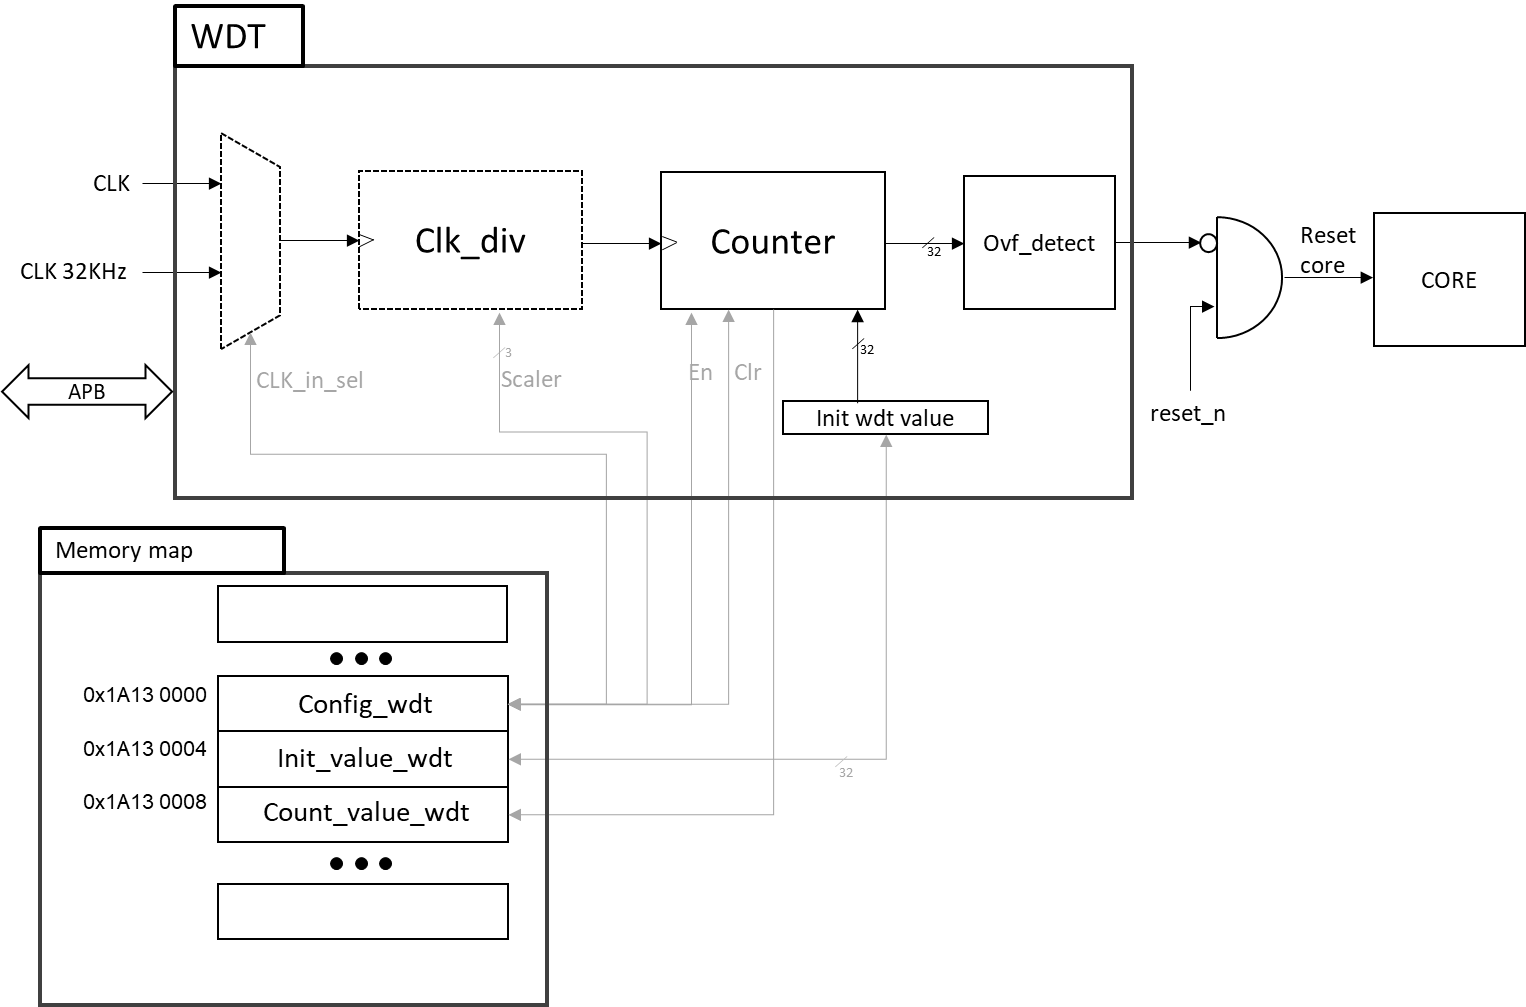
\includegraphics[width=0.9\textwidth]{./figures/wdt.png}
  \caption{WDT block diagram.}
  \label{fig:wdt_overview}
\end{figure}


The following registers can be accessed.

\regDesc{0x1A13\_0000}{0x0000\_0000}{Config wdt}{
  \begin{bytefield}[rightcurly=.,endianness=big]{32}
  \bitheader{31,30,29,28,27,26,25,24,23,22,21,20,19,18,17,16,15,14,13,12,11,10,9,8,7,6,5,4,3,2,1,0} \\
  \begin{rightwordgroup}{CONF}
    \bitbox{26}{- - -}
    \bitbox{1}{\tiny Clk}
    \bitbox{3}{\tiny Presc}
    \bitbox{1}{\tiny Clr}
    \bitbox{1}{\tiny En}
  \end{rightwordgroup}\\
  \end{bytefield}
}{
  \regItem{R/W register}{}{
	CONF reg bit
    \begin{itemize}
      \item \signal{Bit 0 :} EN (Enable watchdog timer)
	\begin{itemize}
	\item 0 : WDT OFF
	\item 1 : WDT ON
	\end{itemize}

      \item \signal{Bit 1 :} CLR (Clear WDT count)
	\begin{itemize}
	\item 0 : 
	\item 1 : WDT counter cleared at init value. After one cycle the bit goes to 0.
	\end{itemize}

      \item \signal{Bit 4-2 :} PRESC (Prescaler counter)  [TODO!!!]
	\begin{itemize}
	\item 000 : 1:1
	\item 001 : 1:2
	\item 010 : 1:4
	\item 011 : 1:8
	\item 100 : 1:16
	\item 101 : 1:32
	\item 110 : 1:64
	\item 111 : 1:128  
	\end{itemize}

      \item \signal{Bit 5 :} CLK (Clock in WDT counter)
	\begin{itemize}
	\item 0 : clock soc\_peripheral
	\item 1 : clock 32 KHz [TODO!!!]
	\end{itemize}
    \end{itemize}
  }
}


\regDesc{0x1A13\_0004}{0x0000\_0000}{Init WDT counter Value}{
  \begin{bytefield}[rightcurly=.,endianness=big]{32}
  \bitheader{31,30,29,28,27,26,25,24,23,22,21,20,19,18,17,16,15,14,13,12,11,10,9,8,7,6,5,4,3,2,1,0} \\
  \begin{rightwordgroup}{INIT\_WDT\_VALUE}
    \bitbox{32}{Init WDT counter Value}
  \end{rightwordgroup}\\
  \end{bytefield}
}{
  \regItem{R/W register}{Init WDT counter Value}{
    This register holds the init counter value. To calculate the initial value, use the following formula:
      \[ Init\_value = 2^{32} - 10^{9}*\frac{time}{per*pres} \]
      Where: 
      \begin{itemize}
      \item time is the wdt time (second)
      \item per is  the period of main clock (nano second)
      \item pres is the power 2 of prescaler value ( $2^{prescaler}$ )
      \end{itemize}
      Example:
      \begin{itemize}
      \item time = 2s
      \item per = 20ns (50MHz)
      \item pres = 1 (prescaler value = 0)
      \item Init\_value = 4194967296 (0xFA0A1F00)

      \end{itemize}
  }
}

\regDesc{0x1A13\_0008}{0x0000\_0000}{WDT counter Value}{
  \begin{bytefield}[rightcurly=.,endianness=big]{32}
  \bitheader{31,30,29,28,27,26,25,24,23,22,21,20,19,18,17,16,15,14,13,12,11,10,9,8,7,6,5,4,3,2,1,0} \\
  \begin{rightwordgroup}{WDT\_VALUE}
    \bitbox{32}{WDT counter Value}
  \end{rightwordgroup}\\
  \end{bytefield}
}{
  \regItem{R register}{Init WDT counter Value}{
    This register holds the watchdog counter value.
  }
}


